%% This is file `elsarticle-template-1-num.tex',
%%
%% Copyright 2009 Elsevier Ltd
%%
%% This file is part of the 'Elsarticle Bundle'.
%% ---------------------------------------------
%%
%% It may be distributed under the conditions of the LaTeX Project Public
%% License, either version 1.2 of this license or (at your option) any
%% later version.  The latest version of this license is in
%%    http://www.latex-project.org/lppl.txt
%% and version 1.2 or later is part of all distributions of LaTeX
%% version 1999/12/01 or later.
%%
%% The list of all files belonging to the 'Elsarticle Bundle' is
%% given in the file `manifest.txt'.
%%
%% Template article for Elsevier's document class `elsarticle'
%% with numbered style bibliographic references
%%
%% $Id: elsarticle-template-1-num.tex 149 2009-10-08 05:01:15Z rishi $
%% $URL: http://lenova.river-valley.com/svn/elsbst/trunk/elsarticle-template-1-num.tex $
%%
%%\documentclass[preprint, 12pt]{elsarticle}

%% Use the option review to obtain double line spacing
 \documentclass[preprint, review,12pt]{elsarticle}

%% Use the options 1p,twocolumn; 3p; 3p,twocolumn; 5p; or 5p,twocolumn
%% for a journal layout:
%% \documentclass[final,1p,times]{elsarticle}
%% \documentclass[final,1p,times,twocolumn]{elsarticle}
%% \documentclass[final,3p,times]{elsarticle}
%% \documentclass[final,3p,times,twocolumn]{elsarticle}
%% \documentclass[final,5p,times]{elsarticle}
%% \documentclass[final,5p,times,twocolumn]{elsarticle}

%% if you use PostScript figures in your article
%% use the graphics package for simple commands
%% \usepackage{graphics}
%% or use the graphicx package for more complicated commands
%% \usepackage{graphicx}
%% or use the epsfig package if you prefer to use the old commands
%% \usepackage{epsfig}

%% The amssymb package provides various useful mathematical symbols
\usepackage{amssymb}
\usepackage{amsmath}
%% The amsthm package provides extended theorem environments
%% \usepackage{amsthm}

%% The lineno packages adds line numbers. Start line numbering with
%% \begin{linenumbers}, end it with \end{linenumbers}. Or switch it on
%% for the whole article with \linenumbers after \end{frontmatter}.
\usepackage{lineno}

%% natbib.sty is loaded by default. However, natbib options can be
%% provided with \biboptions{...} command. Following options are
%% valid:

\usepackage{bm}

%Griffiths' uses this script r for the separation vector. 

\def\r{{\mbox{$\resizebox{.09in}{.08in}{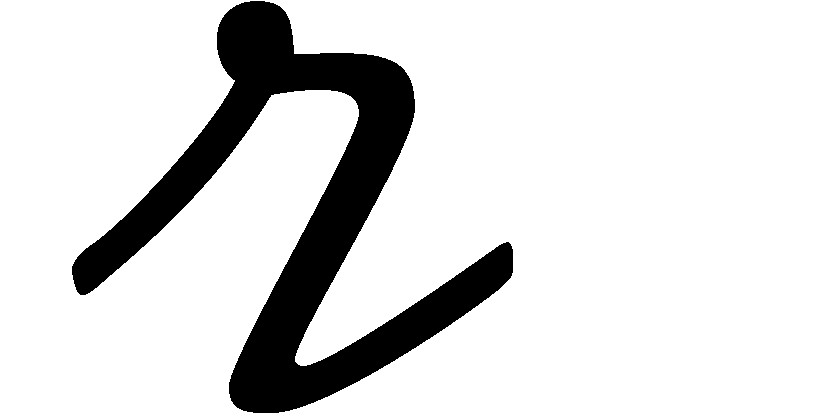
\includegraphics[trim= 1em 0 14em 0,clip]{images/ScriptR.pdf}}$}}}

\def\br{{\mbox{$\resizebox{.09in}{.08in}{
\includegraphics[trim= 1em 0 14em 0,clip]{images/BoldR.pdf}}$}}}
\def\hr{{\mbox{$\hat \br$}}}

%For use in electrodynamics instead of having to write out these prefactors every time

\def\k{\frac{1}{4 \pi \epsilon_0}}
\def\m{\frac{\mu_0}{4\pi}}
\def\x{\times}
\def\.{\cdot}
\def\b{\textbf}
\def\bell{\bm{\ell}}
\def\={\equiv}
\def\emf{\mathcal{E}}
\def\div{\nabla \.}
\def\curl{\nabla \x}
\def\lap{\nabla^2}
\def\and{\quad \text{and} \quad}
\def\9{\left(}
\def\0{\right)}

\newcommand{\pd}[2]{\frac{\partial #1 }{\partial #2}}
\newcommand{\pds}[2]{\frac{\partial^2 #1 }{\partial {#2}^2}}
\newcommand{\td}[2]{\frac{d #1 }{d #2}}
\newcommand{\tds}[2]{\frac{d^2 #1 }{d {#2}^}}
\newcommand{\tup}[1]{\overset{\text{\tiny $\bm\leftrightarrow $}}{\b #1}}
\newcommand{\hb}[1]{\hat{\b #1}}
\newcommand{\hbm}[1]{\hat{\bm #1}}
\newcommand{\brak}[1]{\langle #1 \rangle}

%%   round  -  round parentheses are used (default)
%%   square -  square brackets are used   [option]
%%   curly  -  curly braces are used      {option}
%%   angle  -  angle brackets are used    <option>
%%   semicolon  -  multiple citations separated by semi-colon
%%   colon  - same as semicolon, an earlier confusion
%%   comma  -  separated by comma
%%   numbers-  selects numerical citations
%%   super  -  numerical citations as superscripts
%%   sort   -  sorts multiple citations according to order in ref. list
%%   sort&compress   -  like sort, but also compresses numerical citations
%%   compress - compresses without sorting
%%
%% \biboptions{comma,round}

% \biboptions{}


\journal{Journal Name}

\begin{document}

\begin{frontmatter}

%% Title, authors and addresses

%% use the tnoteref command within \title for footnotes;
%% use the tnotetext command for the associated footnote;
%% use the fnref command within \author or \address for footnotes;
%% use the fntext command for the associated footnote;
%% use the corref command within \author for corresponding author footnotes;
%% use the cortext command for the associated footnote;
%% use the ead command for the email address,
%% and the form \ead[url] for the home page:
%%
%% \title{Title\tnoteref{label1}}
%% \tnotetext[label1]{}
%% \author{Name\corref{cor1}\fnref{label2}}
%% \ead{email address}
%% \ead[url]{home page}
%% \fntext[label2]{}
%% \cortext[cor1]{}
%% \address{Address\fnref{label3}}
%% \fntext[label3]{}

\title{Electrodynamics}

%% use optional labels to link authors explicitly to addresses:
%% \author[label1,label2]{<author name>}
%% \address[label1]{<address>}
%% \address[label2]{<address>}

\author{Joshua}

%\address{Address}

%\begin{abstract}
%% Text of abstract
%Abstract
%\end{abstract}

\end{frontmatter}

%%
%% Start line numbering here if you want
%%
%%\linenumbers

%% main text

\tableofcontents

\section{Introduction}

I am starting with Griffith's fourth edition of introduction to electrodynamics. I also have volume 1 of the Pauli lectures which goes over electrodynamics. Finally I have Jackson which I do not think I will be using to prep for the qualifying exam. \cite{GriffithsEM} \cite{PauliEM} \cite{Jackson}

I will be skipping mathematical introductions as I will consolidate all of that into a different text at a different time. In this text's current form, I have just been going through Griffiths and copying down a lot of the equations from there. I hope to be able to go back and put more of my voice into these notes once I have finished going over Griffiths' book.

\section{Basic Electrostatics}

\subsection{Coulomb's Law}

The basic approach to electrostatics involves Coulomb's law,

\begin{equation}
    \b{F} = \k\frac{qQ}{\r^2}\hr.
\end{equation}

This approach deals with source charges, which are point like objects that carry some charge, q. $\epsilon_0$ is the permittivity of free space, equal to $8.85 \x 10^{-12} \hspace{3pt} C^2/ N \. m^2 $. This equation is more or less postulating and then checked via experiment. Lets use this as one of our postulates of electrostatics. Once we move to electrodynamics this can be derived from Maxwell's equations. Because this equation is linear with respect to q or Q, then the law of superposition can be used when calculating out the total force on a particular charge.

Another fundamental equation of electrostatics is the definition of the electric field, 

\begin{equation}
    \b{F} \= q\b{E}.
\end{equation}

So combining what we have so far, the electric field for electrostatics is equal to,

\begin{equation}
    \b{E}(\b{r}) = \frac{1}{4 \pi \epsilon_0} \sum_{i=1}^n \frac{q_i}{\r^2} \hr
\end{equation}

This equation can be useful for a small amount of charges, or some very symmetrical cases but for a lot of what is done in electrostatics, you will be facing continuous charge distributions rather than this discrete form.


\subsection{Continuous Charge Distributions}

To deal with continuous charge distributions we have to switch out the summation for an integral and what we are left with is,

\begin{equation}
    \b{E}(\b{r}) = \k \int \frac{1}{\r^2}\hr dq.
\end{equation}

That dq though can be a tricky thing to establish. Usually instead of a dq, you would want it in terms of a distance. We can rewrite dq for the one-dimensional case to be equal to $\frac{dq}{dl} dl$. In problems $\frac{dq}{dl}$ is normally given to you as the linear charge distribution $\lambda$. Similarly for two-dimensions and three-dimensions we have $dq = \frac{dq}{da}da$ and $dq = \frac{dq}{d\tau}d\tau$ respectively. $\frac{dq}{da}$ is normally given as the surface charge density $\sigma$ and $\frac{dq}{d\tau}$ is normally given as the volume charge density $\rho$.


An example, is if you have a long wire, the electric field produced by it would be equal to,

\begin{equation}
    \b{E}(z) = \k \frac{2\lambda}{z} \hb{z}.
\end{equation}

The equations for a sphere and plane will be worked out by me later and added.

\subsection{Gauss's Law}

One of the staples of the theory of electrodynamics is Gauss's law which relates the Electric flux to the enclosed charge. Electric flux is defined by

\begin{equation}
    \Phi_E \= \int_S \b{E}\. d\b{a}.
\end{equation}

Gauss's law states that the electric flux is related to the charge enclosed by

\begin{equation}
    \oint \b{E}\. d\b{a} = \frac{Q_{enc}}{\epsilon_0}.
\end{equation}

From this integral equation we can derive a differential equation,

\begin{equation}
    \div \b{E} = \frac{\rho}{\epsilon_0},
\end{equation}

which is also called Gauss's law. 

Useful results that can be calculated from Gauss's law are uniformly charged symmetrical objects. The electric field for a uniformly charged sphere is,

\begin{equation}
    \b{E}= \frac{1}{4 \pi \epsilon_0} \frac{q}{r^2}\hb{r}.
\end{equation}

For a uniformly charged plane the electric field is,

\begin{equation}
    \b{E} = \frac{\sigma}{2\epsilon_0}\hb{n}.
\end{equation}

\subsection{Conservative Force}

Faraday's law states that for electrostatics, the electric force is conservative. In differential form this means that

\begin{equation}
    \curl \b{E} = 0,
\end{equation}

and in integral form,

\begin{equation}
    \oint \b{E} \. d\b{l} = 0.
\end{equation}

I would like to note that this does not hold for electrodynamics though which will be covered later. Because the electric field is a conservative force we can define a potential to be,

\begin{equation}
    \b{E} \= -\nabla \phi,
\end{equation}

where $\phi$ is the electric potential or scalar potential. This potential is sometimes denoted by V instead of $\phi$ such as in Griffith's textbook.

The integral form of this is

\begin{equation}
    \phi(\b{r}) = - \int_O^r \b{E}\. d \bell.
\end{equation}

Where O is some reference point. O is normally where one defines the zero of the potential and is frequently at infinity. A case where this does not apply is the uniform plane where the electric field is not zero at infinity. 

\subsection{Laplace and Poisson Equations}

To try and simplify some problems, we will want to work with the potential rather than the electric field. To do so we need to convert Faraday's law and Gauss's law to be with respect to the electric potential. Taking Gauss's law and putting it in terms of the potential results in

\begin{equation}
    \lap \phi = -\frac{\rho}{\epsilon_0}.
\end{equation}

This is known as Poisson's equation, and when there exists no source charges then $\rho = 0$ and we get Laplace's equation,

\begin{equation}
    \lap \phi = 0.
\end{equation}

But what happens if we plug the potential into Faraday's law. What results is essentially a tautology because the curl of a gradient is zero. Therefore we only need a single equation to determine all of the physics rather than two.

Since the potential is useful quantity, we should have equations that allow us to solve for it that do not depend on the electric field. Taking the equation for a continuous charge distribution in three dimensions and substituting in the definition of the potential results in

\begin{equation}
    \phi(\b{r}) = \k \int \frac{\rho(\b{r'})}{\r}d\tau'.
\end{equation}

Sometimes it is quicker to derive the potential using this equation and then the field from that rather than jumping to the field directly. 

\subsection{Boundary Conditions}

Electric fields always have a jump discontinuity at surface charges. How much the electric field changes depends on what component you are looking at. For the perpendicular component

\begin{equation}
    E_{above}^\bot - E_{below}^\bot = \frac{\sigma}{\epsilon_0},
\end{equation}

and for the parallel component,

\begin{equation}
    E_{above}^\parallel = E_{below}^\parallel.
\end{equation}

The potential on the other hand does not have jump discontinuities because if it did then the electric field would be infinite at that point. Instead we can use our definition of the potential and put it into the equation that has the discontinuity to get back

\begin{equation}
    \pd{\phi_{above}}{n} - \pd{\phi_{below}} = -\frac{\sigma}{\epsilon_0}.
\end{equation}

I have used the notation of a normal derivative without explaining it yet. The $\frac{\partial \phi}{\partial n}$ is a normal derivative and is defined as such

\begin{equation}
    \pd{\phi}{n} = \nabla \phi \. \hb{n},
\end{equation}

where $\hat{n}$ is the normal to the boundary. 


\subsection{Work and Energy}

The work it takes to move a charge from point a to point b is given by can be derived from the definition of work which is,

\begin{equation}
    W \= \int_a^b \b{F}\. d\bell.
\end{equation}

Taking it from there and substituting the previous discussions ideas results in

\begin{equation}
    W = q[\phi(\b{b})-\phi(\b{a})]
\end{equation}

Now let b be an arbitrary vector $\b{r}$ and let a be the reference point for where the potential is equal to zero. Then the work function takes on a different meaning and is just the potential energy of the system. Algebraically this means,

\begin{equation}
    U = q\phi(\b{r}),
\end{equation}

where U is the potential energy of the system of this single particle.

For a collection of particles the the potential energy is

\begin{equation}
    U = \frac{1}{2}\sum_{i=1}^n q_i \phi(\b{r}_i).
\end{equation}

The half comes from the fact that the sum double counts every interaction.

But so far all of this has been for discrete systems. What if we are dealing with the much more realistic continuous systems? Well through some mathematical manipulation the equation becomes 

\begin{equation}
    U = \frac{\epsilon_0}{2}\int E^2 d\tau, 
\end{equation}

where the bounds of integration are all of space.

\subsection{Conductors}

In insulators electrons must stay with their respective atoms while in conductors the electrons are free to move about. Dielectric is just another name for an insulator. Most everyday materials are either conductors or insulators. 

Some of the useful properties of a conductor are that the electric field inside a conductor is zero. This means that the charge density is also zero and the potential is some constant. More useful properties are that all the charge resides on the surface and the surface is equipotential. Lastly because of the boundary conditions, the electric field just outside a conductor must be perpendicular to the conductor's surface. 

An example of applying these principles would be for a neutral conductor that has a cavity in the middle of it. Then since it is neutral, any charge that's in the cavity must have an equal and opposite charge on the outside shell of the conductor due to Gauss's law. From this you could calculate the electric field outside the conductor, or even within the cavity.

Surface charges on a conductor will experience a force equal to 

\begin{equation}
    \b{f} = \frac{\sigma^2}{2 \epsilon_0} \hb{n}.
\end{equation}

Therefore there is an outward electrostatic pressure on the pressure equal to

\begin{equation}
    P = \frac{\epsilon_0}{2}E^2
\end{equation}

\subsection{Capacitors}

Capacitance is defined to be

\begin{equation}
    C \= \frac{Q}{\phi},
\end{equation}

and is measured in farads. This quantity is a purely geometrical one. For a parallel-plate capacitor, each of area A and distance d apart, the voltage

\begin{equation}
    \phi = \frac{Q}{A\epsilon_0}d,
\end{equation}

and thus the capacitance is,

\begin{equation}
    C = \frac{A\epsilon_0}{d}.
\end{equation}

What is the capacitance for two concentric spherical metal shells, with radii a and b is another example that is somewhat frequent. For this it can be found that

\begin{equation}
    C = 4\pi \epsilon_0 \frac{ab}{b-a}.
\end{equation}

Another thing important for capacitors is the energy stored in one. The work to charge up a capacitor is

\begin{equation}
    W = \frac{1}{2}C \phi^2
\end{equation}

\section{Potentials}

\subsection{Laplace's Equation}

Solutions to the Laplace equation come in the form of harmonic functions. For one dimension the general solution is simply

\begin{equation}
    \phi(x) = mx + b
\end{equation}

Properties of the one dimensional case that generalize to the two and three dimensional case are,

\begin{equation}
    \phi(x) = \frac{1}{2}[\phi(x+a) + \phi(x-a)],
\end{equation}

and the solutions have no local maxima or minima; the extrema occur at the end points. 

Earnshaw's Theorem states that a charged particles cannot be held in a stable equilibrium by electrostatic forces alone.

\subsection{Boundary Conditions}

You need boundary conditions to fully specify the solution to Laplace's equation. First uniqueness theorem states that the solution to Laplace's equation in some volume V is uniquely determined if $\phi$ is specified on the boundary surface S. Therefore the potential in a volume V is uniquely determined if the charge density throughout the region and the value of $\phi$ on all boundaries is specified. The second uniqueness theorem states that in a volume V surrounded by conductors and containing a specified charge density $\rho$, the electric field is uniquely determined if the total charge on each conductor is given.

\subsection{Method of Images}

Because of the uniqueness theorems we can devise a clever way to solve some problems that have a symmetry about them. If we are given some boundary conditions for $\phi$, usually involving some long grounded planes. By putting opposite charged charges in the correct locations, you can get the same boundary value problem. From the uniqueness theorem, the solutions to the two different problems must be the same. Therefore you just solve the simpler case with Coulomb's law and call it groovy.

For the example of a single charge +q that is located a distance d above an infinite grounded plane, 

\begin{equation}
    \phi(x,y,z) = \frac{1}{4 \pi \epsilon_0}(\frac{q}{\sqrt{x^2+y^2+(z-d)^2}} + \frac{-q}{\sqrt{x^2+y^2+(z+d)^2}})
\end{equation}

From here you can derive the induced charge distribution $\sigma$, which comes out to be

\begin{equation}
    \sigma(x,y) = \frac{-qd}{2\pi (x^2+y^2+d^2)^{\frac{3}{2}}}
\end{equation}

and thus the total induced charge must be -q. Note that the force can also be calculated from the method of images BUT you can not use the method of images to calculate the energy of the problem. For this problem the energy stored would only be half of the image problem,

\begin{equation}
    U = -\k\frac{q^2}{4d}
\end{equation}

\subsection{Multipole Expansion}

What is the potential for some $\rho \neq 0$ but $Q_{enc} = 0$? Well For cases of multipoles, and for the time being, dipoles, we can calculate it using the multipole expansion. To lay out the problem, what is the potential far away from two equal and opposite charges which are separated at a distance d from each other?

To start out with you would take the explicit formula for the potential would be 

\begin{equation}
    \phi(\b{r}) = \frac{1}{4\pi \epsilon_0}(\frac{q}{r_+}+\frac{-q}{r_-}).
\end{equation}

The next step is to expand out the $r_\pm$.

\begin{equation}
    r_\pm = r^2 + (d/2)^2 \mp rd\cos\theta.
\end{equation}

By using Taylor expansions and other basic approximation techniques you should end up at

\begin{equation}
    \phi(\b{r}) \cong \k \frac{qd\cos\theta}{r^2}
\end{equation}

A trick to see if your calculation is trick to see if your solution is correct, the potential should fall of like $\frac{1}{r^{n+1}}$ where n is the power of your pole. So for a hexadecapole, which is $2^4$ pole, then should fall off like $\frac{1}{r^5}$.

The general equation for the multipole expansion is

\begin{equation}
    \phi(\b{r}) = \frac{1}{4\pi \epsilon_0} \sum_{n=0}^\infty \frac{1}{r^{n+1}} \int (r')^n P_n(\cos \alpha ) \rho(\b{r}')d\tau'.
\end{equation}


Explicitly writing out the monopole and dipole terms,

\begin{equation}
    \phi_{mon}(\b{r}) = \k \frac{Q}{r},
\end{equation}

and,

\begin{equation}
    \phi_{dip}(\b{r}) = \frac{1}{4 \pi \epsilon_0}\frac{1}{r^2}\hat{r}\. \int \b{r'}\rho(\b{r'})d\tau'.
\end{equation}

In the dipole term, the integral is called the dipole moment, and is defined as

\begin{equation}
    \b{p} \= \int\b{r'} \rho(\b{r'})d\tau'.
\end{equation}

Using this definition we can rewrite the dipole's contribution as

\begin{equation}
    \phi_{dip}(\b{r}) = \k\frac{\b{p}\. \hb{r}}{r^2}.
\end{equation}

Note that for physical dipoles, $\b{p} = q\b{d}$ where $\b{d}$ is the separation vector between the positive and negative points.

\section{Electric Fields in Matter}

\subsection{Dipoles}

When a neutral object such as an atom in placed into an electric field, the electrons are pushed in one direction while the nucleus is pulled in the opposite. Even though the overall charge is neutral, the atom now becomes a dipole. This is what we mean when we say an electric field induces a dipole. When this happens we say the atom is polarized. If the field is not too strong the dipole moment is proportional to the field,

\begin{equation}
    \b{p} = \alpha \b{E}.
\end{equation}

The proportionality constant $\alpha$ is called the atomic polarizability, which is a measured quantity. For a more general case, $\alpha$ is not a scalar but actually a tensor called the polarizability tensor.  


What about for polar molecules? Well if a molecule already has some polarization $\b{p}$ then it will experience a torque when placed inside the external electric field. This torque is equal to 

\begin{equation}
    \b{N} = \b{p} \x \b{E}.
\end{equation}

This torque forces $\b{p}$ to be in the same direction as $\b{E}$. If the field is not uniform there exists a net force on the object equal to 

\begin{equation}
    \b{F} = (\b{p} \. \nabla)\b{E}.
\end{equation}

The energy of an ideal dipole in an external electric field is

\begin{equation}
    U = - \b{p} \. \b{E}.
\end{equation}

\subsection{Polarization}

So if you put a dielectric material in an electric field, what will happen is that each molecule in the material will become polarized with a polarization $\b{p}$. When examining the bulk material it is easier to look at the dipole moment per unit volume, $\b{P}$, or polarization.

To answer the question of what type of field this produces, we need to define a surface charge density and a volume charge density. Let the surface charge density be defined as 

\begin{equation}
    \sigma_b \= \b{P} \. \hb{n},
\end{equation}

and the volume charge density defined as,

\begin{equation}
    \rho_b \= - \div \b{P}.
\end{equation}

Using these definitions, and the formula for the potential defined earlier, you can derive

\begin{equation}
    \phi(\b{r}) = \k\oint_S \frac{\sigma_b}{\r}da' + \k \int_v \frac{\rho_b}{\r}d\tau'.
\end{equation}

So to calculate the potential, and thus the electric field, all one needs to do is examine what happens to the bound charges. What is a bound charge though? Is it math or a physical reality. Well as Griffiths puts it, "there is nothing further from the truth" than viewing these bound charges as mathematical constructs. It is called bound charges because they can not be removed from their source unlike a metal. They are a bulk feature, of many dipoles cancelling each other out and just looking at what the overall effect is. 

\subsection{Electric Displacement Field D}

So now we want to examine how the field due to bound charges interacts with everything else. We shall attribute the name free charge, or $\rho_f$ so the "everything else." From how we defined free charge we can use that definition to say

\begin{equation}
    \rho = \rho_b + \rho_f.
\end{equation}

Now incorporating this definition into Gauss's law leads to

\begin{equation}
    \epsilon_0 \div \b{E} = - \div \b{P} + \rho_f
\end{equation}

Defining a new variable, the electric displacement,

\begin{equation}
    \b{D} \= \epsilon_0 \b{E} + \b{P},
\end{equation}

then allows us to rearrange the equation to be,

\begin{equation}
    \div \b{D} = \rho_f.
\end{equation}

The integral form of this is

\begin{equation}
    \oint \b{D} \. d\b{a}= Q_{f_{enc}}
\end{equation}

Boundary conditions for the electric displace are as follows,

\begin{equation}
    D_{above}^\bot - D_{below}^\bot = \sigma_f
\end{equation}

\begin{equation}
    \b{D}_{above}^\parallel - \b{D}_{below}^\parallel = \b{P}_{above}^\parallel - \b{P}_{below}^\parallel.
\end{equation}

\subsection{Dielectrics}

Just like in the atomic case, when an electric field, which is not too strong, is applied to some materials, then the polarization is proportional to the field,

\begin{equation}
    \b{P} = \epsilon_0 \chi_e \b{E}.
\end{equation}

The new proportionality constant $\chi_e$ is called the electric susceptibility, and if a material obeys this equation it is called a linear dielectric. If we were to convert the equation for electric displacement with this equation, then we would derive 

\begin{equation}
    \b{D} = \epsilon_0 (1+\chi_e)\b{E} = \epsilon \b{E}.
\end{equation}

This new constant of proportionality, $\epsilon$, is called the permittivity of the material. From this we can define can also define a new variable, the relative permittivity ( or dielectric constant ), 

\begin{equation}
    \epsilon_r \= 1 + \chi_e = \frac{\epsilon}{\epsilon_0}
\end{equation}

If the space is entirely filled with a homogeneous linear dielectric then this simplifies a lot of our problems because now electric displacement would be irrotational. In general though, dielectrics are not isotropic. In the general case, $\chi_e$ is actually a tensor called the susceptibility tensor. 

For homogeneous linear isotropic materials, the bound charge density can be related to the free charge density by

\begin{equation}
    \rho_b = - \frac{\chi_e}{1+\chi_e}\rho_f
\end{equation}

To compute the energy in a dielectric system, applying the definitions applied above, simplifies the equation down to

\begin{equation}
    U = \frac{1}{2}\int \b{D}\. \b{E} \hspace{4pt} d\tau.
\end{equation}

This equation ONLY works for linear homogeneous isotropic dielectrics though.

For the special case of a finite parallel plate capacitor, with separation d, and width $w$, the force felt on the dielectric by the fringing fields is equal to 

\begin{equation}
    F = -\frac{\epsilon_0\chi_ew}{2d}\phi
\end{equation}

\section{Magnetostatics}

\subsection{Lorentz Law}

For electrostatics we required stationary charges, and for magnetostatics we will require steady currents.. The fundamental force law of magnetostatics is called the Lorentz force law. This law was experimentally found so I will write it as a definition,

\begin{equation}
    \b{F}_{mag} \= q(\b{v} \x \b{B}).
\end{equation}

Combining this with the definition of the electric field results in the full electrodynamics force equation,

\begin{equation}
    \b{F} = q(\b{E} + \b{v} \x \b{B}).
\end{equation}

The v in this equation is the velocity of the particle moving. I guess I should say now that the "magnetic forces do no work" just to go ahead and get that out of the way. Since they do no work, the motion of a particle under just a magnetic force is a circle. Thus using equation the magnetic force to the centripetal force you can get the cyclotron formula,

\begin{equation}
    B = \frac{mv}{qR}.
\end{equation}

The cyclotron frequency is thus

\begin{equation}
    \omega = \frac{QB}{m}.
\end{equation}

Another way of rewriting the Lorentz law in terms of current

\begin{equation}
    \b{F}_{mag} = I \bell \x \b{B}.
\end{equation}

Instead of just talking about one dimensional currents, there are two dimensional surface currents, and three dimensional volume currents. For two dimensional currents we define them as

\begin{equation}
    \b{K} \= \frac{d\b{I}}{d\ell_\bot} = \sigma \b{v},
\end{equation}

and for three dimensional currents,

\begin{equation}
    \b{J} \= \frac{d\b{I}}{da_\bot} =\rho \b{v}.
\end{equation}

The continuity equation stemming from charge conservation is

\begin{equation}
    \div \b{J} = - \frac{\partial \rho}{\partial t}.
\end{equation}

\subsection{Biot-Savart Law}

The Biot-Savart law is

\begin{equation}
    \b{B}(\b{r}) = \m \int \frac{\b{I} \x \hat{\r}}{\r^2}dl' = \m I \int \frac{d\bell \x \hr}{\r^2}.
\end{equation}

Here I have introduced a new constant, $\mu_0$, which is called the permeability of free space. Unless you are trying to be more precise than $10^{-16}$, you can simply use $\mu_0 = 4\pi \x 10^{-7} H/m$.

An example of using this would be finding the magnetic field a distance s from a long straight wire that has a current I. The magnetic field is then,

\begin{equation}
    \b{B} = \frac{\mu_0I}{2\pi s}\hbm{\phi}.
\end{equation}

Another common example is to find the magnetic field a distance z above the center of a circular loop of radius R, carrying a steady current I. In this case the magnetic field is

\begin{equation}
    \b{B}(\b{z}) = \frac{\mu_0I}{2} \frac{R^2}{(R^2+z^2)^\frac{3}{2}}\hb{z}.
\end{equation}

\subsection{Ampere's Law}

So we have arrived at another of Maxwell's equations, Ampere's law. Maxwell will add a correction to this equation later on but in the magnetostatics case Ampere's law works just fine. Ampere's law is analogous to Gauss's law for magnetostatics. Written in integral form it is,

\begin{equation}
    \oint \b{B} \. d\b{l} = \mu_0 I_{enc},
\end{equation}

while written in differential form is,

\begin{equation}
    \curl \b{B} = \mu_0 \b{J}.
\end{equation}

Like Gaussian surfaces, these one dimensional loops are called Amperian loops. This is one of the staples of magnetostatics to be able to calculate the magnetic field due to some current. 

Now the divergence of the magnetic field is fairly simple, simpler in fact than the electrostatics case. This is also one of Maxwell's equations, and is

\begin{equation}
    \div \b{B} = 0.
\end{equation}

All this is saying is that in nature, there does not exist magnetic point charges, i.e. magnetic monopoles. 

\subsection{Magnetic Vector Potential}

For electrostatics we took advantage of the fact that $\curl \b{E} = 0$ to define a scalar potential. Now for magnetostatics we will take advantage of $\div \b{B} = 0$ to define a vector potential. vector calculus identities allow us to define a vector such that,

\begin{equation}
    \b{B} = \curl \b{A}.
\end{equation}

One of the features of this vector potential is that we can define it in such a way that it is divergenceless. Now this is picking a particular gauge is called the Coulomb gauge, or radiation gauge. What is this gauge I'm referencing? Well a gauge is just a systematic way to set a fixed point in a potential, usually the zero. There are other gauges, such as the Lorenz gauge which can be useful for relativistic problems that we will explore later. Converting some of the previous equations into forms dependent on the vector potential we get,

\begin{equation}
    \lap \b{A} = - \mu_0 \b{J},
\end{equation}

and,

\begin{equation}
    \b{A}(\b{r)} = \m \int \frac{\b{J(\b{r'})}}{\r}d\tau'.
\end{equation}

\subsection{Boundary Conditions}

Just like for electrostatics we have some boundary conditions for the magnetic field at boundaries. Very creative wording there. Anyways, 

\begin{equation}
    B_{above}^\bot = B_{below}^\bot
\end{equation}

is the boundary condition for the perpendicular component of the magnetic field. Note that this is analogous to the boundary condition for the parallel portion of the electric field. For the parallel portion of the magnetic field,

\begin{equation}
    B_{above}^\parallel - B_{below}^\parallel = \mu_0 K.
\end{equation}

This reminds me of the perpendicular portion of the electric field! The boundary conditions for the magnetic and electric fields essentially flipped versions of each other. To combine the magnetic field boundary equations into a single vector equation

\begin{equation}
    \b{B}_{above} - \b{B}_{below}= \mu_0 (\b{K} \x \hb{n}).
\end{equation}

\subsection{Multipole Expansion}

Harking back to electrostatics again, the magnetic vector potential can be written in terms of a multipole expansion. To show what it looks like

\begin{equation}
    \b{A}(\b{r}) = \m I \sum_{n=0}^\infty \frac{1}{r^{n+1}}\oint (r')^n  P_n(\cos\alpha) d\bell '.
\end{equation}

Now something to note is that THERE IS NO MAGNETIC MONOPOLE as we stated earlier thus the first term always vanishes. So the first non-vanishing term is the dipole term which is

\begin{equation}
    \b{A}_{dip}(\b{r}) = \m \frac{\b{m} \x \hb{r}}{r^2},
\end{equation}

where $\b{m}$ is the magnetic dipole moment, which is defined to be

\begin{equation}
    \b{m} \= I\b{a}.
\end{equation}

$\b a$ is the vector area of the loop, which for most simple cases is $a\hb{n}$. From this we can derive what the magnetic field due to a dipole must be

\begin{equation}
    \b{B}_{dip}(\b{r}) = \m \frac{1}{r^3}[3(\b{m} \. \hat{r})\hat{r} - \b{m}].
\end{equation}

\section{Magnetic Fields in Matter}

\subsection{Dipoles}

What do we mean when we call something magnetized? This is just lay speak for saying something is magnetically polarized. There are three main types of ways an object can be magnetized. First there are paramagnets which have a magnetization in the same direction of $\b B$, diamagnets which are in the opposite direction of $\b B$, and ferromagnets whose direction is based off the history of magnetic fields that have been applied over time, not just the current one.

All of these stem from the electrons moving around atoms, creating magnetic dipoles. Each of these dipoles has a magnetic dipole moment $\b m$ and just like for electric dipoles the torque on one of these is

\begin{equation}
    \b N = \b m \x \b B.
\end{equation}

Also similarly the force on a magnetic dipole in a inhomogeneous magnetic field is

\begin{equation}
    \b F = \nabla (\b m \. \b B).
\end{equation}

If you apply these equations to an atom, then carrying through the calculations you end up with $\b m$ being in the opposite direction of $\b B$. This is what is responsible for diamagnetism. This effect is much weaker than paramagnetism, but is present in all materials. So when paramagnetism is not present, usually with atoms with an even number of electrons, diamagnetism is the leading order effect.

\subsection{Magnetization}

Another analogous term to the study of electric fields is when we talk about bulk magnetization. For electrostatics there is $\b P$, and for magnetostatics there is $\b M$ which is the magnetic dipole moment per unit volume, and is called the magnetization. Now using this definition in the equation for the vector potential from atomic magnetizations, we can define bound currents just like we defined bound charges. 

\begin{equation}
    \b J_b \= \curl \b M,
\end{equation}

is a bound volume current while

\begin{equation}
    \b K_b \= \b M \x \hb{n},
\end{equation}

is a bound surface current. From this the equation for the vector potential becomes

\begin{equation}
    \b A(\b r) = \m \int_V \frac{\b J_b(\b r')}{\r}d\tau' + \m \oint_S \frac{\b K_b(\b r')}{\r} da'.
\end{equation}

\subsection{Auxillary Field H}

Just like in electrostatics there is a secondary field that takes account for the magnetization of the material. For magnetostatics this field is called the auxillary field and is denoted by $\b H$. Following the same derivation that was done for electrostatics we will split up the current into the bound and free portions,

\begin{equation}
    \b J = \b J_b + \b J_f.
\end{equation}

Then using the definition of $\b J_b$ we used earlier and solving for $\b J_f$ we arrive at 

\begin{equation}
    \curl ( \frac{1}{\mu_0}\b B - \b M) = \b J_f.
\end{equation}

Now we can use this to define the auxillary field,

\begin{equation}
    \b H \= \frac{1}{\mu_0} \b B - \b M.
\end{equation}

Thus the differential form of Ampere's law in terms of the auxillary field is

\begin{equation}
    \curl \b H = \b J_f,
\end{equation}

and the integral form is

\begin{equation}
    \oint \b H \. d \bell = I_{f_{enc}}.
\end{equation}

\subsection{Effects of Media}

For electrostatics we had a name for this, namely the dielectric. Magnetization does not have a good name for the effect of the actual material. What we can talk about though is the property the material changes, which is the magnetic susceptibility and permeability. Just like before, for fields that are not strong, most materials behave in a linear fashion. Unlike in electrostatics we will define the magnetic susceptibility through the auxiliary field,

\begin{equation}
    \b M = \chi_m \b H.
\end{equation}

$\chi_m$ is called the magnetic susceptibility. Just like in electrostatics though we can define a new constant $\mu$ such that

\begin{equation}
    \mu \= \mu_0(1+\chi_m),
\end{equation}

and we will call it the permeability of the material. We can thus draw the parallel to bound volume charge being proportional to free volume current through the equation

\begin{equation}
    \b J_b = \chi_m \b J_f.
\end{equation}

\section{Electrodynamics}

Everything we have done so far has consisted of either static charges or steady currents. What if this is not the case though? Well an interesting phenomena arises that allows us to combine the theory of the electricity and magnetism into one, electromagnetism. This is where the fun begins!

\subsection{Ohm's Law}

So from beginner electromagnetism courses, there is the familiar Ohm's law

\begin{equation}
    V = IR.
\end{equation}

But how does this fit into the vector formalism that we have been using so far? Well, that formula stems from the more general formula

\begin{equation}
    \b J = \sigma \b E,
\end{equation}

where $\sigma$ represents the conductivity of the material. How one determines the conductivity of a material is by testing the resistance $\rho$ (or more likely just looking it up in a table) and then taking the reciprocal, $1/\rho = \sigma$. For conductors $\rho = 0$ and for insulators $\rho = \infty$.

To get the more familiar version of Ohm's law, one just uses the geometry of a given problem, and you can find the value of R algebraically in terms of $\sigma$. From this more familiar Ohm's law you can get Joule heating law which is

\begin{equation}
    P = IV = I^2R.
\end{equation}

\subsection{Faraday's Law}

In a circuit currents are pushed through the wires and circuit elements by some force $\b f$. This force can be split up into two parts, source force of course\footnote{Yes I purposely wrote it this way because it is funny to say out loud. I do not mean to be condescending with my use of "of course."} such as a battery, and an electrostatics force that helps keep the current equal in all areas. Electromotive force is defined as the line integral of the total force around the circuit

\begin{equation}
    \emf \= \oint \b f \. d\bell = \oint \b f_s \. d\bell.
\end{equation}

The reason we are able to drop the $\b E$ from the integral is because $\oint \b E \. d \bell = 0$. For an ideal source $\b E = - \b F_s$ and thus $V = \emf$.

One source of emf is motion inside a magnetic field. This will lead us back to the more recognizable equation for emf. Let us define the magnetic flux to be

\begin{equation}
    \Phi = \int \b B \. d\b a.
\end{equation}

Then the emf is equal to 

\begin{equation}
    \emf = - \td{\Phi}{t}.
\end{equation}

This is called the flux rule for motional emf. A series of experiments by Faraday showed the induced emf was the same when moving the magnetic field to the left or the wire to the right. He also showed that changing the magnetic field could cause an emf. Combining these three facts he stated that a changing magnetic field induced an electric field. Mathematically this is represented by

\begin{equation}
    \curl \b E = - \pd{\b B}{t},
\end{equation}

in its differential form, and in its integral form

\begin{equation}
    \oint \b E \. d \bell  = - \int \pd{\b B}{t} \. d\b a = -\td{\Phi}{t}.
\end{equation}

A handy way to keep track of signs when using Faraday's law is to invoke Lenz's law which states "nature abhors a change in flux."

From Faraday's law we can make an analog to the Biot-Savart law, now for electrostatics

\begin{equation}
    \b E = - \frac{1}{4 \pi} \pd{}{t} \int \frac{\b B \x \hr}{\r ^2}d\tau.
\end{equation}

To calculate $\b B$ for this equation, you might be tempted to use magnetostatics even though the magnetic field is changing. This is fine for most cases except for electromagnetic waves or radiation. This regime is called quasistatic case. 

\subsection{Inductance}

Imagine you have two different loops, and you run a current through one of the loops. This would cause a magnetic field, $\b B_1$, to be created which will interact with the second loop. This second loop then has some magnetic flux. This magnetic flux can be calculated through the simple equation

\begin{equation}
    \Phi_2 = M_{21}I_1.
\end{equation}

This new variable $M_{21}$ is called the mutual inductance between the two loops. This can be calculated from the not so useful Neumann formula

\begin{equation}
    M_{21} = \m \oint \oint \frac{d \bell_1 \. d \bell_2}{\r}.
\end{equation}

While this isn't the most useful formula it does teach us a few things about mutual inductance. Firstly it is a purely geometrical quantity depending on the line integrals, and that $M_{21} = M_{12}$.

But to be honest, that part isn't to interesting in its current form. Like why would I add it to the electrodynamic chapter if I was just going to talk about a magnetostatics phenomena? Well here is the kicker, if I now vary the current through loop one over time, then I am changing the magnetic flux through the second loop and causing an emf to occur! But that induces a current in the second wire which is going to produce its own magnetic field which will then interact with the first loop. And guess what! That is going to cause another emf to be produced! How exciting, I'm sure everyone will have tons of fun calculating this all out.

To simplify the thought experiment, what if our two loops were just the same loop. When we run a changing current through the loop, it causes a magnetic field to be produced which causes a magnetic flux within the same loop. Varying this current would cause an emf to occur which is trying to fight the change in current we are supplying to the loop. This is what back emf is, because nature abhors a change in magnetic flux, then you have to provide a little extra juice to get the current you want. Self equation for self inductance boils down to

\begin{equation}
    \emf = -L\td{I}{t},
\end{equation}

where L is just some geometric quantity which can often be solved by solving

\begin{equation}
    \frac{\Phi}{I} = L.
\end{equation}

Can we calculate how much work must be done to combat this back emf? Also where does the energy go? Well the work done is 

\begin{equation}
    W = \frac{1}{2}LI^2. 
\end{equation}

This work is actually just the energy stored in the magnetic field. When the circuit is turned back off, all this energy is taken away from the field and put back into trying to maintain the flow of current. A generalization of the previous equation is 

\begin{equation}
    W = \frac{1}{2 \mu_0} \int B^2 d\tau,
\end{equation}

where the bounds of integration are over all space. This represents the total energy stored in a magnetic field. 

\subsection{Maxwell's Equations}

So at this point, I've identified four main equations throughout the text which I have referenced as Maxwell's equations in some capacity. Also all the equations have been attributed to other scientist, why is the set of them attributed to Maxwell? Why is it taking me till now to organize them all together? Well I will answer all of these questions now. You might notice an oddity in the current set of Maxwell equations. Namely, that a changing magnetic field induces an electric but not vice versa. Well this is where our homie Maxwell comes in and saves the day. Ampere's law in its current form does not not work for nonsteady current. This is because the divergence of Ampere's law states that $\mu_0 \div \b J = 0$ which does not hold true in general. Adding a quick fix to this results in a new equation

\begin{equation}
    \curl \b B = \mu_0 \b J + \mu_0 \epsilon_0 \pd{\b E}{t}.
\end{equation}

Maxwell called this fix the displacement current and defined it as 

\begin{equation}
    \b J_d \= \epsilon_0 \pd{\b E}{t} = \pd{\b D}{t}.
\end{equation}

Now connecting all of the different phenomena and adding this fix fully unifies electricity and magnetism together. We can take these four equations as axioms for theoretical classical electrodynamics. If we include in another axiom, the Lorentz force law, then we can derive the rest of classical electrodynamics. Pretty nifty huh? Well we can push the symmetry of these equations even further if we assumed magnetic monopoles do exist. Then Maxwell's equations would read

\begin{equation}
\begin{split}
        & \div \b E  = \frac{\rho_e}{\epsilon_0}, \hspace{25.50pt} \curl \b E  = -\mu_0 \b J_m - \pd{\b B}{t} \\
        & \div \b B  = \mu_0 \rho_m, \quad  \curl \b B  = -\mu_0 \b J_e - \mu_0\epsilon_0\pd{\b E}{t}\\
\end{split}
\end{equation}

The e and m subscripts are to differentiate electric vs magnetic charges and currents.Having the equations in this way fixes a lot of the symmetry problems but is unphysical. So I will not talk about the what-if scenario of magnetic monopoles existing further.\footnote{I personally do believe in the existence of magnetic monopoles, but the I do not feel like they are relevant to the discussion of classical electrodynamics.}
    
\section{Conservation law}

We have run into a conservation law already, the continuity equation,

\begin{equation}
     \pd{\rho}{t} = -\div \b J.
\end{equation}

This tells us that there is a local charge conservation, and this is baked into Maxwell's equations. Remember, I said that the only axioms we need are Maxwell's equations and the Lorentz force law, so the local continuity of charge must stem from just those five equations. We want to derive similar equations for all of the other quantities that are normally conserved such as energy, momentum, and angular momentum.


\subsection{Conservation of Energy}

We have already run into the equation for energy in electric and magnetic fields independently earlier. Harking back to them

\begin{equation*}
    W_e = \frac{\epsilon_0}{2} \int E^2 d\tau \and W_m = \frac{1}{2\mu_0} \int B^2 d\tau.
\end{equation*}

Thus the energy density is

\begin{equation}
    u = \frac{1}{2}(\epsilon_0 E^2 + \frac{1}{\mu_0} B^2).
\end{equation}

This is only one half of a continuity equation though as it represents an energy "charge" density. What is the energy "current?" Well from Maxwell's equations we can derive Poynting's theorem,

\begin{equation}
    \td{W}{t} = - \td{}{t} \int_V \frac{1}{2}(\epsilon_0 E^2 + \frac{1}{\mu_0} B^2) d\tau - \frac{1}{\mu_0} \oint_S (\b E \x \b B) \. d\b a.
\end{equation}

This is simply an analogy to the work energy theorem of classical mechanics. If we look at the second integral, we can define a new vector called the Poynting vector equal to

\begin{equation}
    \b S \= \frac{1}{\mu_0} (\b E \x \b B).
\end{equation}

This represent an energy flux density or energy "current." Thus combining the two quantities in this section we can create the continuity equation for energy

\begin{equation}
    \pd{u}{t} = - \div \b S.    
\end{equation}

\subsection{Conservation of Momentum}

If you look strictly at the particles in electrodynamics, it would appear they violate momentum conservation. For classical theories, this is strictly not allowed though. So what's the catch? We have to take into account the momentum carried by the fields themselves. 

To carry out the calculations needed we are going to define the Maxwell stress tensor.\footnote{When I was first learning about this tensor my group of friends all joked that is called the Maxwell stress tensor because of how much stress it causes to undergraduates haha.} When I first was introduced to it I thought it was just a big nasty mess. Let's define the Maxwell stress tensor as

\begin{equation}
    T_{ij} \= \epsilon_0 (E_iE_j - \frac{1}{2}\delta_{ij}E^2) + \frac{1}{\mu_0}(B_iB_j - \frac{1}{2}\delta_{ij}B^2).
\end{equation}

Using this object we can write the total electromagnetic force on a set of charges as 

\begin{equation}
\label{mompoyn}
    \b F = \oint_S \tup{T} \. d\b a - \epsilon_0 \mu_0 \td{}{t} \int_V \b S \hspace{3.5pt} d\tau.
\end{equation}

This shows us that the Maxwell stress tensor is like a momentum "current". It is interesting to note that the current of a vector is a tensor, while the current of scalar is a vector. Thus by using the fact that the force is simply the time derivative of the momentum we can write Equation \ref{mompoyn} as 

\begin{equation}
    \td{\b p_{mech}}{t} = -\epsilon_0 \mu_0 \td{}{t}\int_V \b S \hspace{3.5pt} d\tau + \oint_S \tup{T} \. d\b a.
\end{equation}

Comparing this to Poynting's equation we can identify what the momentum density should be,

\begin{equation}
    \b g = \mu_0\epsilon_0 \b S.
\end{equation}

I would like to note again that since the quantity we are dealing with, momentum, is a vector, its density is also a vector. Now we can write the continuity equation for momentum to be

\begin{equation}
    \pd{\b g}{t} = \div \tup{T}.
\end{equation}

From here we can define angular momentum from the usual means as 

\begin{equation}
    \b L = \b r \x \b g.
\end{equation}

Angular momentum unfortunately does not have a nice neat and tidy continuity equation.\footnote{:(.}

\section{Electromagnetic Waves}

\subsection{Electromagnetic Waves in Vacuum}

Decoupling Maxwell's equations leads to two three dimensional wave equations

\begin{equation}
    \lap \b E = \mu_0 \epsilon_0 \pds{\b E}{t}, \and \lap \b E = \mu_0 \epsilon_0 \pds{\b B}{t}.
\end{equation}

From the knowledge of wave mechanics we know that $\mu_0 \epsilon_0$ is a speed of propagation of the wave and we can see that both the electric and magnetic fields travel at this speed. If we are to plug in their values we find that

\begin{equation}
    \frac{1}{\sqrt{\mu_0 \epsilon_0}} = 3.00 \x 10^8 m/s.
\end{equation}

This is actually just the speed of light. This implies that light is an electromagnetic wave. From plugging the solutions of the wave equation into Maxwell's equation we find that 

\begin{equation}
    \b B = \frac{1}{c} \hb{k} \x \b E,
\end{equation}

where $\b k$ is the wave vector. This implies that the phase of the electric and magnetic fields are the same and that the fields are perpendicular to each other. 

Plugging this equation back in Poynting vector results in

\begin{equation}
    \b S = \frac{1}{\mu_0c}E^2\hb{k} = c\epsilon_0 E^2 \hb{k} = cu \hb{k},
\end{equation}

where u is the energy per unit volume. Also by how we defined the momentum density, it must be equal to 

\begin{equation}
    \b g = \frac{u}{c} \hb{k}
\end{equation}

Time averaging these values results in

\begin{equation}
\begin{split}
    & \brak{u} = \frac{\epsilon_0}{2}E^2, \\
    & \brak{\b S} = \frac{c\epsilon_0}{2}E^2 \hb{k}, \\
    & \brak{\b g} = \frac{\epsilon_0}{2c}E^2 \hb{k}.
\end{split}
\end{equation}

Let us define the intensity of an electromagnetic wave as 

\begin{equation}
    I \= \brak{\b S \. \hb{k}}.
\end{equation}

Thus when electromagnetic waves comes into contact with something there is some sort of radiation pressure. For a perfect absorber there this radiation pressure is equal to 1/c, and for a perfect reflector the radiation pressure is 2/c.

All of these results transfer over to if light is placed in matter with the simple switch of $\epsilon_0 \rightarrow \epsilon$ and $\mu_0 \rightarrow \mu.$ The speed of the wave then is 1/$\sqrt{\mu \epsilon}$ = c/n where n is the index of refraction. If $\mu_r$ is not given in the problem you should assume it to be 1.

\subsection{Reflection and Transmission of EM Waves}

When talking about the reflection and transmission of waves let a subscripts I, R, T represent the incident, reflected, and transmitted portions of the quantities. If the plane comes at a boundary at normal incidence then the reflection coefficient is 

\begin{equation}
    R \= \frac{I_R}{I_I} = (\frac{n_1 - n_2}{n_1+ n_2})^2,
\end{equation}

where I is the is intensity of the wave. The transmission coefficient\footnote{These are very similar to a lot of wave mechanics problems such as in classical mechanics or quantum mechanics.} is

\begin{equation}
    T \= \frac{I_T}{I_I} = \frac{4n_1n_2}{(n_1 + n_2)^2}.
\end{equation}

Notice how R+T = 1, which states that all of the quantities, such as energy and momentum, of the incident wave are exactly accounted for in the reflected and transmitted waves. But does all of this hold for oblique incidence? There are three laws of optics which we must take into account when talking about this.

The first law states that the incident, reflected, and transmitted wave vectors form a plane which also include the normal to the surface. What this tells me, that if I take any two of those vectors that are linearly independent, then I have a basis that I can write the other two vectors in terms of.

The second and third law relate different angle to each other. The second law, or law of reflection, states that the angle of incidence is equal to the angle of reflection. Lastly the third law, also known as Snell's law or the law of refraction, is an equation relating the incident angle to the transmitted angle,

\begin{equation}
      n_1 \sin\theta_I = n_2\sin\theta_T.
\end{equation}

Now let us define two new coefficient $\alpha$ and $\beta$

\begin{equation}
    \alpha \= \frac{\cos\theta_T}{\cos\theta_I},
\end{equation}

and

\begin{equation}
    \beta \= \frac{\mu_1n_2}{\mu_2n_1}.
\end{equation}

This allows us to concisely write Fresnel's equations for polarization in the plane of incidence. 

\begin{equation}
    E_{0_R} = \9 \frac{\alpha - \beta}{\alpha + \beta} \0 E_{0_I}, \and E_{0_T} = \9\frac{2}{\alpha + \beta}\0 E_{0_I}.
\end{equation}

Solving this for normal incidence we can recover the formula for Brewster's angle which in the most general form is

\begin{equation}
    \sin^2\theta_B = \frac{1-\beta^2}{(n_1/n_2 -\beta^2}.
\end{equation}

Making the assumption that $\mu_r$ for both material is roughly equal to one allows us to recover the simplified version of Brewster's angle

\begin{equation}
    \tan\theta_B = \frac{n_2}{n_1}.
\end{equation}

\subsection{Absorption and Dispersion of Electromagnetic Waves}

 All of that is fine and dandy, but what if there actually is free charges and currents? For conductors free charges and free charge currents will spread out and form a charge distribution on the surface almost instantaneously. Maxwell's equations then become
 
\begin{equation}
\begin{split}
    & \div \b E = 0, \quad \curl \b E = -\pd{\b B}{t}, \\
    & \div \b B = 0, \quad \curl \b B = \mu \epsilon \pd{\b E}{t} + \mu \sigma \b E.
\end{split}
\end{equation}

If we try to put these into wave equation form a new term arises

\begin{equation}
    \lap \b E = \mu \epsilon \pds{\b E}{t} + \mu \sigma \pd{\b E}{t}, \and \lap \b B = \mu \epsilon \pds{\b B}{t} + \mu \sigma \pd{\b B}{t}.
\end{equation}

All that new term changes is the wave number in the plane wave solution to become 

\begin{equation}
    {k'}^2 = \mu \epsilon\omega^2 + i \mu \sigma \omega = k + i\kappa.
\end{equation}

We define k and $\kappa$ to be

\begin{equation}
     k \= \omega\sqrt{\frac{\epsilon\mu}{2}} \9 \sqrt{1 + \9 \frac{\sigma}{\epsilon\omega} \0^2} + 1 \0^{\frac{1}{2}},
\end{equation}

and

\begin{equation}
    \kappa \= \omega\sqrt{\frac{\epsilon\mu}{2}} \9 \sqrt{1 + \9 \frac{\sigma}{\epsilon\omega} \0^2} - 1 \0^{\frac{1}{2}}.
\end{equation}

Now when discussing optics a useful quantity that emerges is the skin depth which is kind of like the time constant for depth of penetration into a conductor. The amplitude of your wave will decrease by a factor of 1/e every

\begin{equation}
    d \= \frac{1}{\kappa}.
\end{equation}

If we are instead to write the complex wave vector like

\begin{equation}
    k' = Ke^{i \phi},
\end{equation}

then we could find out some interesting physical phenomena about the fields inside the conductor. 

First lets define K and $\phi$;

\begin{equation}
    K \= \omega \sqrt{\epsilon \mu \sqrt{1 + \9 \frac{\sigma}{\epsilon\omega} \0^2}},
\end{equation}

and 

\begin{equation}
    \phi \= \tan^{-1} \frac{\kappa}{k}.
\end{equation}

Plugging these quantities back into the initial differential equation we see that the magnetic field lags behind the electric field by a factor of $\phi.$ Also the proportionality factor between the fields isn't just c/n, but actually

\begin{equation}
    \frac{B_0}{E_0} = \sqrt{\epsilon \mu \sqrt{1 + \9 \frac{\sigma}{\epsilon\omega} \0^2}}.
\end{equation}

Looking at these equation we can see that there is a problem for perfect conductors where the charge density is infinite. In this case the wave is completely reflected and picks up a phase shift of $\pi$.

\subsection{Frequency Dependence of Permittivity}

So far we have assumed that $\epsilon$ and $\mu$ are just strictly scalar quantities. In general though they are more complicated, and one of these complication is that they change depending on the frequency of the light passing through the material. We can thus model them as scalar functions. Physically what happens is the electrons will get excited by different frequencies, and these different excitations cause different levels of damping to occur. We will model electrons as springs. In doing so we can then define the macroscopic polarization $\b P$ to be the real part of

\begin{equation}
    \b P = \frac{Nq^2}{m} \9 \sum_j \frac{f_j}{w_j^2 - w^2 - i \gamma_j \omega} \0 \b E.
\end{equation}

Here I have used $f_j$ as the different electrons which have natural frequency $\omega_j$, and damping $\gamma_j$. This complex polarization is proportional to the complex field which allows us to define it through the normal means as well

\begin{equation}
    \b P = \epsilon_0 \chi_e' \b E,
\end{equation}

where $\chi_e'$ is the complex susceptibility. Using the manipulations we had before results in a complex dielectric constant

\begin{equation}
    \epsilon_r' = 1 + \frac{Nq^2}{m} \9 \sum_j \frac{f_j}{w_j^2 - w^2 - i \gamma_j \omega} \0.
\end{equation}

Looking at this equation we can see that the damping only plays a large role around the natural frequencies of the electrons. We can go through the same tricks as the last subsection and get monochromatic plane waves as solutions to the boundary conditions. Now we will define the absorption coefficient as 

\begin{equation}
    \alpha \= 2 \kappa,
\end{equation}

which tells us about how much the wave will become attenuated. Around the resonance the index of refraction will drop suddenly, and this phenomena is called the anomalous dispersion. In this region the material will actually become almost opaque.

If we stay away from resonance and look at transparent media, which normally have natural frequencies in the ultraviolet we can then get the formula for the index of refraction to be 

\begin{equation}
    1 + \9 \frac{Nq^2}{2m\epsilon_0} \sum_j \frac{f_j}{\omega_j^2} \0  + \omega^2 \9 \frac{Nq^2}{2m\epsilon_0} \sum_j \frac{f_j}{\omega_j^4} \0.
\end{equation}

Then we can define new variables A and B to make this take the form of Cauchy's formula

\begin{equation}
    n = 1 + A \9 1 + \frac{B}{\lambda^2} \0.
\end{equation}

A is the coefficient of refraction while B is the coefficient of dispersion and this formula works best for most gases in visible wavelengths.

\subsection{Guided Waves}

Instead of infinite plane waves, what if our electromagnetic wave is confined to be in some wave guide. For this discussion we will assume the wave guide is a perfect conductor and thus we will use the boundary conditions of such. From working out the solutions to the boundary conditions it becomes apparent that the waves can not be strictly transverse and have some longitudinal component. In fact the transverse components can be found if we only know the longitudinal component. Let us assume that the wave is moving in the $\hb z$ direction. Then we can write the the transverse components as 

\begin{equation}
\begin{split}
    & E_x = \frac{i}{(\omega/c)^2 - k^2} \9 k \pd{E_z}{x} + \omega \pd{B_z}{y} \0, \\
    & E_y = \frac{i}{(\omega/c)^2 - k^2} \9 k \pd{E_z}{y} - \omega \pd{B_z}{x} \0, \\
    & B_x = \frac{i}{(\omega/c)^2 - k^2} \9 k \pd{B_z}{x} + \frac{\omega}{c^2} \pd{E_z}{y} \0, \\
    & B_y = \frac{i}{(\omega/c)^2 - k^2} \9 k \pd{B_z}{y} - \frac{\omega}{c^2} \pd{E_z}{x} \0.
\end{split}
\end{equation}

Plugging all of this back into Maxwell's equation results in two coupled equations

\begin{equation}
\begin{split}
    & \9 \pds{}{x} + \pds{}{y} + (w/c)^2 - k^2 \0 E_z = 0, \\
    & \9 \pds{}{x} + \pds{}{y} + (w/c)^2 - k^2 \0 B_z = 0.
\end{split}
\end{equation}

From here we can now define what TE, TM, and TEM waves are. If the $E_z = 0$, then it is a TE (transverse electric) wave, if $B_z = 0$ then it is a TM (transverse magnetic) wave, and if it is both then it is a TEM wave. TEM waves cannot happen if you are in a hollow wave guide. 

When solving for TE waves in a rectangular wave guide, then the magnetic component will be of the form

\begin{equation}
    B_z = B_0 \cos(m\pi x/a)\cos(n \pi y/b),
\end{equation}

which then will be denoted as the TE$_{mn}$ mode. The first index is conventionally related to the bigger of the two dimensions. One of the two indices must be nonzero for TE waves. If the frequency of the light is less than some cutoff frequency $\omega_{mn}$ defined to be

\begin{equation}
    \omega_{mn} \= c \pi \sqrt{(m/a)^2 + (n/b)^2},
\end{equation}

then the wave will attenuate exponentially. For the example we are working with, the lowest cutoff frequency is 

\begin{equation}
    \omega_{10} = c \pi /a.
\end{equation}

A useful visualization that you c an do in your head is that the electromagnetic wave is travelling at some angle with the wave guide and bouncing back and forth. The allowed wavelengths are those that produce standing waves in the x-y plane. 

An example of when TEM waves are allowed is a coaxial cable. In the solution for the TEM waves, it reduces back down to electrostatics and magnetostatics. Thus this example has already been solved and the solution is simply

\begin{equation}
\begin{split}
    & \b E = \frac{A\cos(kz-\omega t)}{s}\hb{s}, \\
    & \b B = \frac{A\cos(kz-\omega t)}{cs}\hbm{\phi}.
\end{split}
\end{equation}

\section{Radiation}

We shall define radiation in this section as the process of the fields taking energy off to infinity due to charges accelerating. Let us say the power radiated through some surface is the surface integral of the Poynting vector, and thus

\begin{equation}
    P(r,t) = \oint \b S \. d \b a = \frac{1}{\mu_0} \oint (\b E \x \b B) \. d\b a.
\end{equation}

We want to evaluate this power at the time $t_0$, but these waves left the center at a time $t_0 + \frac{r}{c}$. Thus 

\begin{equation}
    P_{rad}(t_0) = \lim_{r\to\infty} P \9 r, t_0 + \frac{r}{c} \0.
\end{equation}

For this value to be finite\footnote{In this context finite means non-zero.} then the fields must fall off faster than 1/r. Since this is not the case in electrostatics nor magnetostatics, there is no radiation to be had. It is only in the electrodynamic case that they arise. 

\subsection{Dipole Radiation}

For this section we are trying to avoid accelerating point charges in favor of dipoles because they are much easier to work with. The model we will use is we have some charges driven between two metal spheres connected by a wire. Let the driving force make the charge move like

\begin{equation}
    q(t) = q_0 \cos(\omega t).
\end{equation}

Thus the dipole moment is 

\begin{equation}
    \b p(t) = p_0 \cos(\omega t) \hb{z},
\end{equation}

where 

\begin{equation}
    p_0 \= q_0d.
\end{equation}

The current through the wire is

\begin{equation}
    \b I(t) = -q_0 \omega \sin(\omega t) \hb{z}.
\end{equation}

If we keep causality in mind, and make the following three approximations, 

\begin{equation}
    d \ll r, \and d \ll \frac{c}{\omega}, \and \frac{c}{\omega} \ll r,
\end{equation}

then we find the potentials to be

\begin{equation}
    \phi(r, \theta, t) = -\frac{p_0 \omega}{4 \pi \epsilon_0 c} \9 \frac{\cos \theta}{r} \0 \sin[\omega(t-r/c)],
\end{equation}

and\footnote{I actually don't use the last approximation in this equation.}

\begin{equation}
    \b A(r, \theta, t) = -\frac{\mu_0 p_0 \omega}{4 \pi r} \sin[\omega(t-r/c)] \hb{z}.
\end{equation}

The first approximation was to try and move away from physical dipoles to perfect dipoles. The second approximation just comes from the fact that the frequency is related to distance by the wavelength of the light, and the wavelength is much larger than d. The last approximation is because we are looking at radiation the radiation zone, which for us is towards infinity.

From the potentials the fields can be directly calculated and thus

\begin{equation}
    \b E = - \frac{\mu_0 p_0 \omega^2}{4 \pi} \9 \frac{\sin\theta}{r} \0 \cos[\omega(t-r/c)] \hbm{\theta},
\end{equation}

and

\begin{equation}
    \b B = - \frac{\mu_0 p_0 \omega^2}{4 \pi c} \9 \frac{\sin\theta}{r} \0 \cos[\omega(t-r/c)] \hbm{\phi}.
\end{equation}

Now we can finally calculate what the Poynting vector is

\begin{equation}
    \b S(\b r, t) = \frac{\mu_0}{c} \9 \frac{p_0 \omega^2}{4 \pi} \9 \frac{\sin\theta}{r} \0 \cos[\omega(t-r/c)] \0^2 \hb{r}.
\end{equation}

Time averaging this quantity results in

\begin{equation}
    \brak{\b S} = \9 \frac{\mu_0 p_0^2 \omega^4}{32\pi c} \0 \frac{\sin^2 \theta}{r}\hb{r},
\end{equation}

which finally allows us to find what the average radiation. Taking the formula we established at the beginning of the section

\begin{equation}
    \brak{P} = \frac{\mu_0 p_0^2 \omega^4}{12 \pi c}.
\end{equation}

\subsection{Magnetic Dipole Radiations}

Instead of the model we used last time, lets just have a wire in the shape of a circle with radius b, and current 

\begin{equation}
    I(t) = I_0 \cos\omega t.
\end{equation}

The magnetic dipole is then 

\begin{equation}
    \b m(t) = m_0 \cos(\omega t) \hb{z},
\end{equation}

where I have defined $m_0$ to be

\begin{equation}
    m_0 \= \pi b^2 I_0.
\end{equation}

I would like to note that the total charge on the loop is zero and thus the scalar potential is zero as well. Using the same approximations as last time but now b plays the role of d, we can solve for the magnetic vector potential. The result is

\begin{equation}
    \b A(r, \theta, t) = - \frac{\mu_0 \omega}{4 \pi c} \9 \frac{\sin\theta}{r} \0 \sin[\omega (t-r/c)] \hbm{\phi}.
\end{equation}

From here we calculate the field directly and the result is

\begin{equation}
    \b E = \frac{\mu_0 m_0 \omega^2}{4 \pi c}\cos[\omega(t-r/c)] \hbm{\phi},
\end{equation}

and

\begin{equation}
    \b B = - \frac{\mu_0 m_0 \omega^2}{4 \pi c^2} \9 \frac{\sin\theta}{r} \0 \cos[\omega(t-r/c)]\hbm{\theta}.
\end{equation}

Following the same method of calculating the average radiation as before we find

\begin{equation}
    \brak{P} = \frac{\mu_0 m_0^2 \omega^4}{12 \pi c^3}.
\end{equation}

I would like to note that this is very similar to the equation for the radiation due to the electric dipole. The main difference is there is an extra factor of $1/c^2$. Therefore if they are both present the electric dipole radiation will be the dominant one. It is only in the special example we have created that there is no electric radiation that the radiation due to magnetic dipoles is important.
























%% The Appendices part is started with the command \appendix;
%% appendix sections are then done as normal sections
%% \appendix

%% References
%%
%% Following citation commands can be used in the body text:
%% Usage of \cite is as follows:
%%   \cite{key}          ==>>  [#]
%%   \cite[chap. 2]{key} ==>>  [#, chap. 2]
%%   \citet{key}         ==>>  Author [#]

%% References with bibTeX database:

\bibliographystyle{model1-num-names}
\bibliography{sample.bib}

%% Authors are advised to submit their bibtex database files. They are
%% requested to list a bibtex style file in the manuscript if they do
%% not want to use model1-num-names.bst.

%% References without bibTeX database:

%\begin{thebibliography}{00}

%% \bibitem must have the following form:
%%   \bibitem{key}...
%%

% \bibitem{}

% \end{thebibliography}

%\appendix

%Appendix

\end{document}

%%
%% End of file `elsarticle-template-1-num.tex'.
